% !TeX root = ../thuthesis-example.tex

\chapter{绪论}
\section{研究背景与意义}
骨髓是人体最主要的造血器官,其存在于人体骨骼内部的空腔中,约占体重的3.5~5.9\%。
作为人体的造血组织,骨髓中包含了多种不同发育阶段的血细胞,
这些血细胞按照形态与功能可以划分为粒细胞系、红细胞系、淋巴细胞系、单核细胞系与浆细胞系。
骨髓血细胞成熟后会通过密质骨中的连通管等进入人体外周血,参与人体循环系统的血液循环,保证机体新陈代谢的进行。

血细胞的质与量出现异常通常与某种血液疾病密切相关。白血病\cite{黄治虎2009我国白血病流行病学调查的现状和对策}是一种常见多发的血液疾病,主要表现为细胞异常克隆增生
导致的骨髓造血功能异常。白血病属于人体造血系统的恶性肿瘤,
在所有恶性肿瘤中占比约5\%,是我国重点防治的十大恶性肿瘤之一。
白血病患者临床症状为贫血、出血、发热、乏力等,其致死率较高,早期发现与治疗对延长患者生存时间、改善患者生活质量至关重要\cite{musto2019update}。

骨髓血细胞形态学检查是精确诊断白血病类型的关键手段之一\cite{heimpel1979conventional}。
目前,大型医院的骨髓血检查主要依靠病理学医师对显微设备采集的血细胞图像进行观察,统计不同类型的
血细胞数量,然后,根据 FAB 分型标准\cite{bennett1976proposals}对白血病类型进行初步诊断。检测流程首先需制备骨髓涂片并使用瑞特与吉氏混合液进行染色。接着,使用低倍显微镜判断骨髓增生程度、
观察是否存在异常形态的特殊细胞。在低倍镜观察完全片后,再使用油镜从骨髓涂片中部向尾部移动,记录约500个有核细胞中各类
血细胞的数量。目前人工镜检存在以下不足,人工分类计数过程非常枯燥且繁琐费时,通常需要数个工作日后才能出具诊断报告,
不能满足快速临床诊疗的需求。对医师的专业技术要求较高,培养精通细胞病理诊断的医师要周期长,年轻医师从事人工镜检的意愿低。
诊断结果依赖于医师的专业知识与经验,存在较强的主观性,诊断的规范性与一致性较差。

在过去的20年间,计算机科学技术高速发展,医疗硬件设备的不断提升,医学领域积累了大量的医疗诊断数据,
人工智能(AI,Artificial Intelligence)技术被广泛应用于医学领域\cite{2018Data,shen2017deep}。目前AI已经在医疗机器人、药物研发、智能问诊、智能影像识别等领域
进行落地与应用。AI高效的计算与分析能力极大提升了医生的工作效率,为疾病检测与诊疗带来了深刻的变革。
在血细胞图像智能诊疗方面,诸多研究学者采用深度学习的方法来自动定位与识别血细胞,实现了快速筛选和分类计数。这项技术使得细胞形态学诊断变的自动化、标准化与智能化,将医生从繁重的细胞病理工作中解放出来,具有非常重要的临床辅助诊断的意义。

目前骨髓血细胞自动化检测与识别技术已取得了长足的进步,但仍然面临着诸多挑战。在血细胞检测方面,涂片背景复杂干扰较多、细胞间相互黏连与重叠会影响检测结果的精确度。
在血细胞识别方面,骨髓血细胞种类非常多,存在各类细胞样本数量不均衡、细胞类内差异大、相邻发育阶段细胞类间差异小等问题。
因此,基于深度学习的血细胞自动检测与识别方法仍有巨大的提升空间。本文针对骨髓血细胞检测与识别关键问题进行研究,并编写相关软件,
为医生的临床诊断提供参考依据,具有非常重要的临床意义与广阔的应用前景。



\section{研究现状与进展}
本节介绍骨髓血细胞检测算法与骨髓血细胞识别算法相关研究现状。
\subsection{骨髓血细胞图像检测现状}
在血细胞涂片图像处理的过程中,包含血细胞区域的提取至关重要,检测与分割结果的精确性对后续识别任务有很大的影响。
如何精准的从血细胞涂片中分割出各类细胞的边界,定位包含血细胞的区域是医学图像处理的重要研究方向之一。
近几十年来,国内外学者对此进行了深入的研究,并提出了多种解决方案,主要可以划分为以下四类,基于阈值的检测方法\cite{1992A,2003A,Wu2006}、
基于边缘检测的方法\cite{Ma2008Novel,Sadeghian2009A}、
基于聚类的检测方法\cite{theera2005white, ramoser2006leukocyte}、
基于深度学习的检测方法。

基于阈值分割方法是一种广泛使用的图像分割技术,其基本思想是在选定的颜色空间中根据某种规则选取一组阈值,
从而将图像分割为不同的区域。常见的阈值选取方法有大津法(OTSU)、分水岭和区域增长方法等。Cseke\cite{1992A}基于OTSU方法,
通过最大化不同色彩区域的类间方差得到分割阈值,实现对细胞核,细胞浆与背景分割,
但该方法对细胞浆的分割结果不尽人意。Jiang\cite{2003A}结合尺度空间滤波与分水岭算法实现对细胞核与细胞浆的分割,
该分割方法首先利用尺度空间滤波从图像中提取出细胞核,然后对三维HSV直方图进行分水岭聚类分割出细胞浆,
该方法对于背景复杂或有噪声的情况下存在过分割的情况。Wu\cite{Wu2006}等利用HIS颜色空间H分量与S分量开发了一种基于圆形直方图的迭代OTSU白细胞分割方法,
该方法在彩色涂片图像上获得了较好的分割结果。

基于边缘检测的方法是是找到图像中变化剧烈的像素点集合,这些点通常是目标的轮廓点。边缘检测借助于表征边缘梯度的边缘算子实现。
常用的边缘算子有Sobel边缘算子、Canny边缘算子等。在血细胞图像中,基于边缘检测的方法对于染色效果好、细胞间无黏连无重叠的区域的分割效果较好,
但在染色欠佳,边界复杂的情况下,很难获得理想的分割结果,该方法通常会结合其他方法来提升图像分割的精度。
马建林\cite{Ma2008Novel}等提出了一种基于边缘检测的区域增长分割算法,该方法首先利用改进的Canny算子进行边缘粗检测,再利用给出的图像灰度值和纹理、颜色等信息进行区域合并,
实验结果表明该方法对于医学图像中的复杂区域与畸形区域具有较强的鲁棒性与实用性。Sadeghian\cite{Sadeghian2009A}等提出了一种基于边缘检测的主动轮廓分割方法,
首先采用Canny算子提取初始的边界,接着利用GVF snake算法以初始边界不断迭代提升轮廓分割的精度。

基于聚类的方法是根据某种相似性规则例如纹理、灰度、颜色等信息将图像中的像素划分为多类,从而实现图像分割。
Theera-Umpon\cite{theera2005white}基于模糊C均值(FCM)将图像过分割为若干小区域,之后计算各个类中心与其他区域中心的关系,
之后将小区域进行合并得到最终的分割结果。模糊C均值的参数依赖于经验值,对于背景复杂,
染色不均的图像难以获得精确的分割结果。Ramoser\cite{ramoser2006leukocyte}使用k-means方法在HSL颜色空间将图像分割为细胞核、
背景、细胞浆-红细胞这三个部分,之后根据初步分割的结果构造白细胞似然图像,
接着应用MSER方法计算分割阈值得到白细胞分割图像。

自2012年,基于深度神经网络的方法在图像分割、图像识别、目标检测等领域取得了巨大的突破并和广泛的应用。
现代的医学图像检测、分割任务几乎都是基于深度学习方法。基于深度学习目标检测可以分类两个流派,两阶段检测与单阶段检测方法,
前者包含一个从粗糙到细致的筛选过程,而后者只需要一步即可完成目标的定位与分类。2014年R. Girshick\cite{girshick2014rich}提出了RCNN模型,
首次将CNN网络应用到目标检测领域。针对RCNN中存在的重叠区域重复计算、图像缩放导致几何形变等问题,何凯明\cite{he2015spatial}、R. Girshick\cite{girshick2015fast}别提出SPP-Net与Fast-RCNN来提高目标检测的运算速度。
2015年,任少卿\cite{ren2015faster}提出了Faster-RCNN网络采用RPN(Region Proposal Network)网络来替代之前的区域推荐方法从而极大提高了目标检测的速度与精度。
单阶段检测器的里程碑是由R. Joseph\cite{redmon2016you}等在2015年提出的YOLO(you only look once)网络,其直接使用单个神经网络用于完整的图像检测,摒弃了双阶段检测器推荐区域与进一步坐标回归和分类的范式。
Lin等\cite{lin2017focal}指出密集检测器在训练期间遇到的前景-背景类别极度不均衡是主要原因,并在此基础上引入了Focal loss,通过重定义标准交叉熵损失函数使得检测器可以将更多的注意力放在困难样本的学习上。
进一步提升了单阶段检测器的检测精度。最近基于Transformer\cite{vaswani2017attention}的模型也被用于目标检测领域,主要可以归纳为以下三种范式,使用Transformer骨干网络替换双阶段目标检测器中的骨干网络来提取图像特征;
使用CNN作为骨干网络提取特征,并将目标检测视为集合预测问题,通过Transformer编码器解码器结构直接输出一组目标的位置与类别信息,代表网络有DETR\cite{zhu2020deformable};
纯粹基于Transformer的端到端目标检测网络,如YOLOS\cite{fang2021you}、PVT\cite{wang2021pyramid}等。基于深度学习的检测网络在通用目标检测数据集(COCO、ImageNet等)取得了优越的性能。诸多研究学者对上述网络进行改进以适用于血细胞涂片图像的目标检测。
Xia\cite{xia2019automated}等使用Faster-RCNN网络进行血细胞检测,检测的准确率达到了98.4\%。
Dhieb\cite{dhieb2019automated}等使用Mask-RCNN网络对红细胞与白细胞进行检测与识别,网络使用在COCO数据集上预训练的Resnet-101网络作为主干网络,并使用FPN网络来提取多尺度的特征用于不同尺寸的细胞检测。
由于训练样本较少,作者采用了多种数据增强方式防止过拟合。该模型对红细胞与白细胞检测准确率分别为92\%与96\%,
并且可以有效的识别重叠和染色欠佳的细胞。
Shakarami\cite{shakarami2021fast}等基于YOLOv3单阶段目标检测网络提出了FED(Fast and Efficient YOLOv3)模型在三个尺度上对血细胞进行检测,
其使用EfficientNet替换Dark-Net53作为主干网络,并应用空洞卷积增加网络的感受野、深度可分离卷积来减小模型的参数量,网络在BCCD数据集上对血小板、红细胞、
白细胞的平均识别准确率分别为90.25\%、80.41\%、98.92\%。

此外,一些研究学者使用基于深度学习的语义分割网络将血细胞图片图像中的细胞分离出来。Ronneberger\cite{long2015fully}等提出了U-Net网络模型,相比于FCN增加了编码器-解码器结构,编码器负责特征提取,解码器将提取的特征进行融合并恢复到原图的尺度。
U-Net网络中使用了跳跃连接将编码器低层级的特征与解码器高层级特征进行拼接从而保留了目标的细节信息,该网络在医学图像分割中获得了良好的性能。
Lu等\cite{lu2021wbc}基于U-Net++和Resnet提出了WBC-Net用于血细胞的分割,WBC-Net设计了一个带有残差模块的特征编码器来提出多尺度特征,
并在密集卷积模块上引入混合跳跃连接来融合不同语义的特征图。WBC-Net使用基于交叉熵和Tversky指数损失函数来训练网络,并获得了98.97\%的分割准确率。
\subsection{骨髓血细胞图像识别现状}
自动血细胞分类技术按照原理可以大致分为以下三类,物理方法、物理-化学方法与图像分析方法\cite{wubai2011}。

物理方法包括了电学与光学方法,其中应用最广泛的是体积-电导-激光散射分析方法(Volume-Conductivity-Scatter),其中体积通过库尔特理论得到,
即包含细胞的电解液通过细小管道时,会导致管道两侧的电阻发生改变,通过这个电信号来确定细胞体积的大小。电导性通过采用高频的探针来探测细胞内部复杂结构,
进而区分杆状核和分叶核。根据激光散射信号的差异来判断细胞质内的颗粒信息,进而区分嗜中性、嗜酸性与嗜碱性细胞。体积-电导-激光检测技术通过对血细胞体积,
细胞核和细胞质颗粒进行分析实现了白细胞精准的五分类,但是仅基于物理的方法无法得到血细胞的形态信息。并且结果容易受到血小板凝集、难溶红细胞等因素的干扰。

物理-化学方法是将细胞化学染色与激光散射相结合的技术。化学染色方法有核酸荧光染色、过氧化酶染色等,在细胞染色后进行激光照射,不同角度的散射光包含了细胞的结构信息,
从而实现对血细胞的分类,但该方法同样不能得到直观的细胞形态学信息。

图像分析方法,骨髓血涂片在经过染色后,不同类型血细胞胞体形状各异且细胞核与细胞浆会呈现出不同的颜色与纹理特征。基于数字图像处理的白细胞分类方法包含了图像采集、图像分割,图像识别这三个部分。
图像采集通常由自动化采集设备完成,首先采用×10倍物镜找到只包含单层细胞的区域,接下来转换到×100倍油镜扫描拍摄该区域得到细胞涂片图像。
图像分割如上节所述,目的是从涂片中定位包含血细胞的区域,得到只包含单个血细胞的切片的图像。图像识别对得到的单个血细胞切片进行分类,
目前主要有两大类方法,基于传统模式识别的分类识别方法和基于深度学习的分类识别方法。

基于传统模式识\cite{jain2000statistical}的血细胞识别方法主要包含特征提取、特征选择与分类器推理预测这三个部分。特征提取是在原始图像中提取出具有区分性的特征,如血细胞的几何形态,色度、纹理、统计等特征。
特征选择对提取到的特征进行可分类能力的评估,从中筛选出最典型的显著特征,剔除无关冗余的特征,从而减少特征数量提升模型的识别速度与精度,常用的特征选择方法有过滤法、
包装法、嵌入法、降维法等。分类器对输入样本的特征集合进行类别预测,分类器的种类非常多,例如朴素贝叶斯、支持向量机、决策树、随机森林,K近邻等。
Ghosh\cite{ghosh2010statistical}等提取了血细胞的面积、周长、圆度、浆核比等九个几何形态特征,并利用t检验方法对特征进行筛选,最终四个显著特征被输入到朴素贝叶斯分类器中,
对五类白细胞的分类准确率为83.2\%。Rezatofighi[30]等提取了形态特征,并基于灰度共生矩阵与局部二值模式提取了纹理特征,
然后采用序列前向选择方法(SFS)对特征进行选择,最后比较了人工神经网络与支持向量机两种分类器的性能。
孙凯\cite{sunkai2020}等提取了几何、纹理、小波三部分共63个特征,在PCA降维后得到了八个主成分,接着使用了支持向量机、多层感知机、决策树对其进行分类,最好的分类结果准确率为88.6\%。
袁满\cite{yuan2017}对细胞核与细胞浆提取了颜色、纹理形态共100个特征,并对提取的特征使用z-score进行标准化,
接着基于Fisher准则选择其中的70个特征,最后使用支持向量机、随机森林和K近邻方法对白细胞进行五分类。

基于传统的机器学习方法依赖专家经验人工设计的特征,无法捕捉高层次的抽象隐含的特征,并且需要进行特征选择来筛选显著性特征,
对于大量的数据样本可能存在模型欠拟合、泛化性能差等缺点,基于深度学习的方法可以实现特征工程的自动化,目前也是血细胞分类识别的主流研究方向。
Matek\cite{matek2019human}等制作了一个包含18375张总计15类的骨髓血细胞图像数据集,针对类别数量不平衡的问题,采用随机0°~360°的旋转变换,与水平翻转垂直扩充训练数据集,
接着采用通用的ResNext网络进行分类,网络对于常见的骨髓血细胞如中性粒细胞、典型淋巴细胞、单核细胞等达到了94\%的识别准确率,该网络没有针对血细胞图像进行改进,
整体的分类准确率不是很理想。Mori\cite{mori2020assessment}将骨髓血细胞按发育不良(细胞质颗粒减少)的程度划分为四类,使用Resnet-152网络对血细胞进行分类,平均灵敏度与特异性分别为85.2\%、98.9\%。
2020年,杭州智微科技\cite{fu2020morphogo}联合陆军军医大学第二附属医院基于2018年到2019年间收集的65986幅真实病例血细胞图片开发出了一个完整的自动化检测识别系统morphogo,该系统可以实现血细胞涂片的自动采集,
检测识别与结果的可视化。该研究使用了27层的卷积神经网络,对于12类骨髓血细胞的分类准确率均超过了85.7\%,但是部分类别的召回率只有40\%,网络的特征表达能力有待提升。
目前市场上的全自动血细胞形态学分析仪比较少,另外一款产品是瑞典CellaVision公司研发DM 96\cite{yoon2019diagnostic}全自动血细胞形态学分析系统,也用于血细胞的预分类辅助医生诊断。
Huang\cite{huang2020attention}等首先基于RetinaNet检测网络得到只包含单个血细胞的切片图像,接着将自适应注意力模块引入到含残差模块的卷积神经网络中,
注意力模块是一个先下采样再上采样的卷积模块,该模块增强了与分类任务相关的区域特征的权重,提升了模型的表达能力,该网络针对六类白细胞实现了95.3\%的平均分类准确率。

\section{本文研究内容}
本文研究所使用的血细胞病理图由邃蓝智能科技(上海)有限公司提供,研究目标是基于深度学习的方法实现骨髓血细胞自动化检测识别
任务,并结合图像采集设备硬件,编写骨髓血细胞自动化检测与识别的软件。软件可将骨髓涂片中血细胞的位置与预分类结果呈现给医生,供其
参考与核对,从而辅助医生临床诊断。本文涉及的内容主要包含基于深度学习的骨髓血细胞检测,骨髓血细胞识别,系统软件解决方案这三个部分。

1)骨髓血细胞检测,本文对比了基于深度学习的单双阶段检测器的速度与精度等性能,并选择在血细胞领域较为先进的RetinaNet作为基线模型。针对密集血细胞区域,血细胞边界框
检测偏差大、黏连细胞边界检测错误等问题,本文在RetinaNet的FPN层后引入了自底向上的路径聚合模块,该模块将更浅层的特征与FPN深层的进行融合,缩短了底层与顶层特征之间的信息传递路径,
使得浅层的纹理等高分辨定位信息可以更容易传递到顶层,提升了网络定位特征的表达能力。我们探究了不同标签分配策略对于检测精度
的影响,并采用基于最优输运的标签分配策略,通过全局最优来解决模糊anchor的分配问题,进一步提升网络的召回能力。最终结合了上述改进方法的检测模型,相较于原有RetinaNet基线模型检测精度有较大提升。

2)骨髓血细胞识别,目前基于深度学习的血细胞识别研究工作主要使用通用的目标分类网络,并未针对血细胞的特性进行改进。此外,很多研究只关注了血细胞大类,未关注其中的子类别如粒细胞的
原始、早幼、中幼与晚幼等阶段,血细胞子类之间差异较小使得其自动化识别更具挑战性。针对上述难点,本文将性能优异的Vision Transformer作为基线模型,提出了
重叠图像块划分方法、辨识性区域选择模块与对比loss对基线模型进行改进。其中重叠图像块划分方法可以更好的保留图像的局部信息、避免破坏图像的局部结构。辨识性
区域选择模块采用压缩激发结构学习所有编码层的注意力图权重,并将每个注意力头最大权重对应的隐含特征用于分类,该模块让网络关注到不同类别之间的细微差异部分,
同时舍弃大量区分度较低的背景、超类共同特征区域,从而提升网络的细粒度特征表达能力。为了进一步增加分类特征的类内一致性与类间差异性。本文引入了对比损失,对特征的间隔进行约束,
使得不同标签特征相似度最小,相同标签的特征相似度最大。本文方法相较于其他卷积神经网络与基线Vision Transformer模型分类准确率有较大提升。

3)骨髓血细胞检测识别系统软件研发,本文通过主动学习的技术完成了一万余张骨髓血细胞图像边界框与类别信息的标注,并完成上述相关检测与
识别算法训练与优化。本文对骨髓血细胞检测与识别软件进行需求分析,确定软件架构为B/S架构,并对数据库各个表单进行详细设计。软件前端使用VUE+ElementUI框架进行
页面设计与交互。后端使用的框架为Python+Django。软件包括了用户登录/注册、骨髓血细胞检测、骨髓血细胞识别、患者信息核查与管理、患者数据分析等五大功能模块。

\section{论文组织结构}
图为本文的组织结构框架,总共分为七个章节,各个章节的详细内容安排如下:

\begin{figure}[htbp]
    \centering
    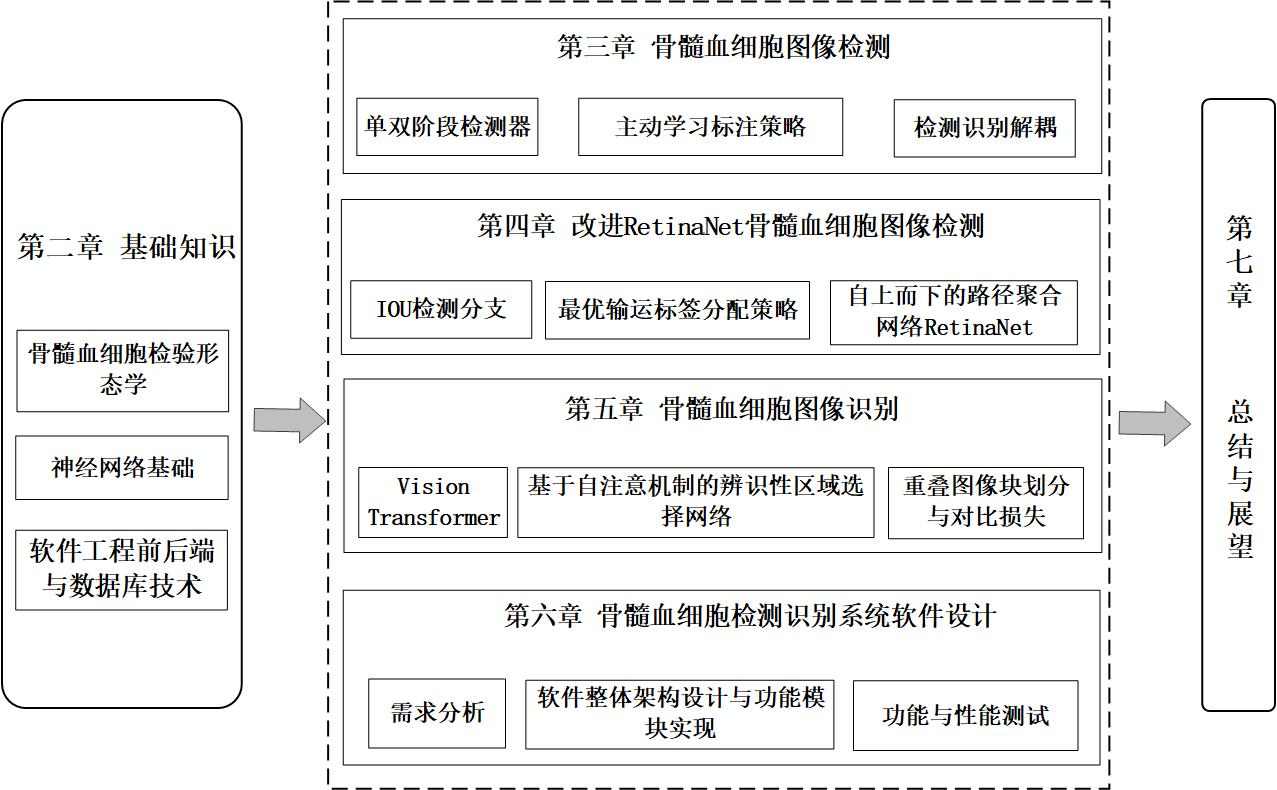
\includegraphics[width=1.0\linewidth]{structure.jpg}
    \caption{论文组织结构}
    \label{fig:structure}
  \end{figure}
  
第一章为绪论。首先介绍了骨髓血细胞形态学检测的背景,并阐述了本文基于深度学习的骨髓血细胞自动化检测与识别的意义。接着,介绍了骨髓血细胞检测与识别的国内外研究现状并
分析各个研究的优势与不足。然后简要说明了本文主要研究内容。最后给出本文的章节组织。

第二章介绍本文的基础知识与技术。本章首先阐述骨髓血细胞相关病理学知识,对比了不同类别骨髓血细胞的形态学差异,介绍骨髓血细胞数据集标注与数据增强方法,并给出了交叉训练集
与测试集的划分。接着,概述神经网络的基本理论与相关检测与识别技术。最后,介绍了软件开发使用的前端、后端与数据库技术。

第三章研究骨髓血细胞检测相关问题。本章对比了多种单阶段与双阶段目标检测网络的检测精度、计算量与速度等性能。并确定将RetinaNet作为为骨髓血细胞检测的基线模型。然后
本章探索了RetinaNet网络在仅检测与检测识别一体化任务上特征提取与识别准确率上的差异,确定了先检测再识别的骨髓血细胞处理流程。

第四章研究基于改进RetinaNet的骨髓血细胞检测网络。针对漏检、误检等问题,在网络结构方面引入了路径聚合网络,缩短底层与顶层特征的信息传递路径,提高网络对
高分辨定位特征的提取能力,减小定位误差。此外引入了引入了IOU预测分支,将检测框的定位质量也纳入到候选框的筛选中。本节对检测网络的标签分配策略进行
研究,提出了一种基于最优输运的全局最优的标签分配策略,提升网络对于血细胞的召回能力与检测精度。

第五章研究骨髓血细胞识别问题。分析了近年来多种基于深度学习的识别网络,提出了一种基于改进Vision Transformer的骨髓血细胞识别模型。
该网络由多个堆叠的自注意编码层组成。为了充分利用自注意力机制,本文采用压缩激发模块学习了多个编码层的注意力权重,该模块可以有效
捕捉到不同细胞之间细微的差异部分,提高网络的细粒度特征表达能力。在训练过程中,将对比损失与交叉熵损失函数进行有机结合,进一步提升网络提取特征的辨识性,该网络模型
在TMAMD骨髓血细胞数据集取得了最佳性能。

第六章介绍骨髓血细胞检测与识别系统软件的设计与实现。本节首先对骨髓血细胞检测识别系统进行需求分析,对软件的开发环境与平台进行说明,
并设计了软件的整体架构。接着详细介绍了数据库表与各个功能模块的设计与实现。最后对软件进行了功能与性能测试,总结了软件的测试结果。

第七章为总结与展望。总结了本文的工作内容,对骨髓血细胞检测与识别的发展进行展望。



